\documentclass[12pt,a4paper]{article}
\usepackage[T1]{fontenc}
\usepackage{textcomp}
\usepackage{makeidx}

\usepackage[sc, noBBpl]{mathpazo}
\usepackage{dsfont} % for indicator function
\usepackage[deluxe]{otf}
\usepackage[utf8]{inputenc}

\usepackage{amsmath}
\usepackage{amsfonts}
\usepackage{amssymb}
\usepackage{amsthm}
\usepackage{mathtools}
\usepackage{mathrsfs}

\usepackage{listings} % for programming codes

\usepackage{bm}
\usepackage[dvipdfmx]{color}
\pagestyle{plain} 
\usepackage{float}
\usepackage[dvipdfmx]{graphicx}

\usepackage[left=15mm, right=18mm, top=20mm, bottom=20mm]{geometry}

\setlength{\footskip}{40pt} 
\setlength{\abovecaptionskip}{0pt}
\setlength{\belowcaptionskip}{0pt}
\renewcommand{\baselinestretch}{1.05}

\newcommand{\argmax}{\mathop{\rm arg max}\limits}
\newcommand{\argmin}{\mathop{\rm arg min}\limits}
\newcommand{\st}{\mathop{\rm s.t.}\limits}
\newcommand{\fsize}[1]{\fontsize{#1}{#1}\selectfont}

% custom color
\usepackage[dvipdfmx]{xcolor}

% colors
\definecolor{darkred}{rgb}{.40,.00,.00}
\definecolor{navy}{rgb}{.00,.00,.40}
\definecolor{darknavy}{rgb}{.00,.00,.30}
\definecolor{lightnavy}{rgb}{.10,.10,.40}

\newcommand{\navy}{\color{navy}}
\newcommand{\deepred}{\color{darkred}}
\newcommand{\emred}[1]{\textbf{\deepred #1}}
\newcommand{\emblue}[1]{\textbf{\navy #1}}

% title and tableofcontents
\usepackage[titles]{tocloft}
\setlength{\cftbeforesecskip}{2pt}
\setlength{\cftbeforesubsecskip}{0pt}
\renewcommand{\cftsecfont}{\normalsize\mcfamily}
\renewcommand{\cftsubsecfont}{\normalsize\mcfamily}
\renewcommand{\cftsubsecfont}{\normalsize\mcfamily}
\renewcommand{\contentsname}{\large\mcfamily\bfseries \S\hspace{0.5\baselineskip}Contents\\[-\baselineskip]}
\cftsetindents{section}{10.0pt}{15.0pt}
\cftsetindents{subsection}{20.0pt}{30.0pt}
\cftpagenumbersoff{section}
\cftpagenumbersoff{subsection}
\cftpagenumbersoff{subsubsection}

\makeatletter
\def\vhrulefill#1{\leavevmode\leaders\hrule\@height#1\hfill \kern\z@}
\makeatother

\makeatletter
\def\maketitle{%
	\begin{center}\leavevmode
	\normalfont
	{\normalsize\raggedleft \@date\par}%
	\vskip -0.7\baselineskip
	\vhrulefill{0.2pt}\par
	\vskip 0.3\baselineskip
	\renewcommand{\baselinestretch}{0.80}
	{\color{darknavy}\bfseries\Large\raggedright \@title\par}%
	\renewcommand{\baselinestretch}{1.00}
	\vskip 0.2\baselineskip
	\ifx\@subtitle\@empty\else%
	{\normalsize\raggedright \@subtitle\par}%
	\fi
	\ifx\@author\@empty\else%
	\vskip 0.5\baselineskip
	{\normalsize\raggedleft \@author\par}%
	\fi
	\end{center}%
	\vskip 1.0\baselineskip
}
\def\subtitle#1{\gdef\@subtitle{#1}}
\let\@subtitle\@empty
\makeatother

% section
\newcommand{\Secindent}{0.0\baselineskip}
\newcommand{\Subsecindent}{0.0\baselineskip}
\newcommand{\lmargini}{1.3\baselineskip}
\newcommand{\lmarginii}{0.5\baselineskip}
\newcommand{\lmarginiii}{0.2\baselineskip}
\def\theenumi{\arabic{enumi}}
\def\theenumii{\alph{enumii}}
\renewcommand{\labelenumi}{\hfill\hspace{60pt}\theenumi.}
\renewcommand{\labelenumii}{\hspace{30pt}\theenumii.}
\renewcommand{\labelitemi}{\small\textbullet\hspace{2pt}}
\renewcommand{\labelitemii}{\color{gray}\small$\circ$\hspace{2pt}}
\renewcommand{\labelitemiii}{\textendash\hspace{1pt}}
\makeatletter
\renewcommand{\section}{\@startsection%
	{section}{1}{\Secindent}% name, depth, indent \z@=0pt
	{-1.0\baselineskip \@plus1.5\baselineskip \@minus0.5\baselineskip}% beforeskip (no indent if negative)
	{0.5\baselineskip \@plus0.8\baselineskip \@minus0.3\baselineskip}% afterskip (no line break if negative)
	{\reset@font\large\bfseries\scshape\color{darknavy}}% font
}
\renewcommand{\subsection}{\@startsection%
	{subsection}{2}{\Subsecindent}%
	{-0.5\baselineskip \@plus0.7\baselineskip \@minus0.4\baselineskip}%
	{0.3\baselineskip \@plus0.5\baselineskip \@minus0.2\baselineskip}%
	{\reset@font\normalsize\bfseries\scshape\color{darknavy}}% 
}
\renewcommand{\thesection}{\@arabic\c@section} % arabic, roman, Roman, alph, Alph, fnsymbol
\renewcommand{\thesubsection}{\thesection\hspace{0pt}.\hspace{0pt}\@arabic\c@subsection}
\makeatother

\makeatletter
\def\@listi{%
	\topsep = 0.2\baselineskip
	\partopsep = 0.0\baselineskip
	\parsep = 0.0\baselineskip
	\itemsep = 0.5\baselineskip
	\leftmargin = 1.5zw
	\labelsep = 0.5zw
	\itemindent = 0pt
	\labelwidth\leftmargin \advance\labelwidth-\labelsep
	\listparindent = 0zw
	\rightmargin = 0pt
	\reset@font\normalsize\normalfont
}
\let\@listI\@listi
\@listi
\def\@listii{%
	\topsep = 0.25\baselineskip
	\partopsep = 0.0\baselineskip
	\parsep = 0.0\baselineskip
	\itemsep = 0.3\baselineskip
	\leftmargin = 0.5zw
	\labelsep = .5zw
	\itemindent = 0pt
	\labelwidth\leftmargin \advance\labelwidth-\labelsep
	\listparindent = 0zw
	\rightmargin = 0pt
	\reset@font\normalsize\normalfont%
}
\def\@listiii{%
	\topsep = 0.30\baselineskip
	\partopsep = 0.0\baselineskip
	\parsep = 0.1\baselineskip
	\itemsep = 0.05\baselineskip
	\leftmargin = 1.1zw
	\labelsep = .5zw
	\itemindent = 0pt
	\labelwidth\leftmargin \advance\labelwidth-\labelsep
	\listparindent = 0zw
	\rightmargin = 0pt
	\reset@font\normalsize\normalfont%
}
\def\@listiv{%
	\topsep = 0.0\baselineskip
	\partopsep = 0.0\baselineskip
	\parsep = 0.0\baselineskip
	\itemsep = 0.0\baselineskip
	\leftmargin = 0.9zw
	\labelsep = .5zw
	\itemindent = 0pt
	\labelwidth\leftmargin \advance\labelwidth-\labelsep
	\listparindent = 0zw
	\rightmargin = 0pt
	\reset@font\normalsize\normalfont%
}
\makeatother

\newcommand{\R}{\ensuremath{\mathbb{R}}}
\newcommand{\E}{\ensuremath{\mathbb{E}}}
\newcommand{\V}{\ensuremath{\mathbb{V}}}
\newcommand{\Cov}{\ensuremath{\text{Cov}}}
\newcommand{\N}{\ensuremath{\mathbb{N}}}
\newcommand{\Z}{\ensuremath{\mathbb{Z}}}
\let\epsilon\varepsilon

\let\origitem\item
\renewcommand{\item}{\normalfont\origitem}

\usepackage[%
backref=page,
dvipdfmx,
bookmarks=true,bookmarksnumbered=true,bookmarkstype=toc,
colorlinks=true,
linkcolor=navy,
citecolor=navy,
filecolor=blue,
pagecolor=blue,
urlcolor=blue
]{hyperref}
\AtBeginDvi{\special{pdf:tounicode EUC-UCS2}}

\renewcommand*{\backref}[1]{}
\renewcommand*{\backrefalt}[4]{%
  \ifcase #1 (Not cited.)%
  \or        [#2]%
  \else      [#2]%
  \fi}
 

\title{State space models}
\subtitle{Introduction to dynamical systems~\#11}
\author{Hiroaki Sakamoto}
\date{\today}

\DeclareMathOperator{\vect}{vec}
 
\begin{document}
\maketitle
\tableofcontents

\section{Auto regression models}

\subsection{Random walk}

\begin{itemize}

\item \textbf{Model}
  \begin{itemize}
  \item Consider the following dynamical system:
    \begin{equation}\label{eq:model_random_walk}%
      x_{t} = x_{t-1} + \nu_{t},
      \quad \nu_{t} \sim \mathcal{N}(0,V),
      \quad t = 0, 1, 2, \ldots,
    \end{equation}
  \item Suppose that
    \begin{itemize}
    \item the value of $V$ is unknown to us
    \item we observed a sample path $X_{n}:=(x_{0},x_{1},x_{2},\ldots, x_{n})$
    \end{itemize}
  \item We want to obtain an estimate (i.e., the best guess) of $V$ based on $X_{n}$
  \end{itemize}

\item \textbf{Maximum likelihood estimation}
  \begin{itemize}
  \item What is the value of $V$ that `justifies' the observed data $X_{n}$?
    \begin{enumerate}
    \item for each possible value of $V$, derive the probability of observing $X_{n}$ (density $p(X_{n})$)%, which is a function of $V$, called the likelihood function $L(V;X_{n})$
    \item the maximum likelihood estimator, $\hat{V}$, is the value of $V$
      that maximizes the probability of observing what was actually observed, $X_{n}$
    \end{enumerate}
  \item The density $p(X_{n})$ of $X_{n}=(x_{0},x_{1},x_{2},\ldots, x_{n})$ may be decomposed as
    \begin{equation}\nonumber%\label{eq:}%
      p(X_{n})
      = p(x_{n}|X_{n-1})p(X_{n-1})
      = p(x_{n}|X_{n-1})p(x_{n-1}|X_{n-2})p(X_{n-2})
      = \left(\prod_{t=1}^{n}p(x_{t}|X_{t-1})\right)p(x_{0}),
    \end{equation}
    where \eqref{eq:model_random_walk} implies
    $x_{t}|X_{t-1} \sim \mathcal{N}(x_{t-1},V)$ and thus
    \begin{equation}\nonumber%\label{eq:}%
      p(x_{t}|X_{t-1})
      = \frac{1}{(2\pi)^{\frac{1}{2}}V^{\frac{1}{2}}}e^{- \frac{1}{2}\frac{(x_{t}-x_{t-1})^{2}}{V}}
      \quad \forall t \geq 1
    \end{equation}
    \clearpage
  \item Assuming $p(x_{0})=1$,
    the \emph{likelihood function} (density seen as a function of parameter) is
    \begin{equation}\nonumber%\label{eq:}%
      L(V;X_{n})
      = \prod_{t=1}^{n}\frac{1}{(2\pi)^{\frac{1}{2}}V^{\frac{1}{2}}}e^{- \frac{1}{2}\frac{(x_{t}-x_{t-1})^{2}}{V}}
      = \left(\frac{1}{(2\pi)^{\frac{1}{2}}V^{\frac{1}{2}}}\right)^{n}e^{- \frac{1}{2V}\sum_{t=1}^{n}(x_{t}-x_{t-1})^{2}}
    \end{equation}
  \item The \emph{maximum likelihood estimator} (MLE) of $V$ is
    the one that maximizes $L(V;X_{n})$,
    which for this particular example, is given as
    \begin{equation}\label{eq:MLE_random_walk}%
      \frac{dL(\hat{V};X_{n})}{dV} = 0
      \iff
      \hat{V} = \frac{1}{n}\sum_{t=1}^{n}(x_{t}-x_{t-1})^{2}
    \end{equation}
  \item Remarks:
    \begin{itemize}
    \item $\hat{V}(X_{n})$ is a function of stochastically generated data (different draw of $X_{n}$ yields a different estimate $\hat{V}$)
    \item If you are unlucky, you may observe $X_{n}$ that rarely occurs (without knowing that it is a rare event),
      in which case $\hat{V}(X_{n})$ may significantly deviate from the true value
  \item In theory, however, MLE gives you a fairly `good' estimate of $V$,
    ensuring $\E[\hat{V}(X_{n})]=V$ and $\lim_{n\to\infty}\hat{V}(X_{n}) = V$;
    See \figurename~\ref{fig:random_walk} for an illustration
    \end{itemize}
  \begin{figure}[t]\centering%
    \includegraphics[width=440pt]%
    {figures/fig_random_walk.pdf}
    \caption{%
      Sample paths $X_{n}$ generated from \eqref{eq:model_random_walk} where $V=3$ (left)
      and the maximum likelihood estimator $\hat{V}(X_{n})$ computed as \eqref{eq:MLE_random_walk} (right).
    } 
    \label{fig:random_walk}
  \end{figure} 

  \end{itemize}

\end{itemize}

\clearpage

\subsection{AR1 model}

\begin{itemize}
\item \textbf{Model}
  \begin{itemize}
  \item Consider the following dynamical system
    \begin{equation}\label{eq:model_ar1}%
      x_{t} = ax_{t-1} + b + \nu_{t},
      \quad \nu_{t} \sim \mathcal{N}(0,V),
    \end{equation}
    which is often called the \emph{autoregressive model} of order $1$ (or AR1 model)

  \item Suppose that
    \begin{itemize}
    \item $a$, $b$, $V$ are all unknown to us
    \item we observed a sample path $X_{n}:=(x_{0},x_{1},x_{2},\ldots, x_{n})$
    \end{itemize}
  \item We want to obtain an estimate of unknown parameters $\bm{\theta}:=(a, b, V)$ based on $X_{n}$
  \end{itemize}

\item \textbf{Likelihood function}
  \begin{itemize}

  \item Model~\eqref{eq:model_ar1} implies that
    the probability density of observing $X_{n}$ is
    \begin{equation}\nonumber%\label{eq:}%
      p(X_{n})
      = \left(\prod_{t=1}^{n}p(x_{t}|X_{t-1})\right)p(x_{0})
      = \left(\frac{1}{(2\pi)^{\frac{n}{2}}V^{\frac{n}{2}}}e^{- \frac{1}{2}\sum_{t=1}^{n}\frac{(x_{t}-ax_{t-1}-b)^{2}}{V}}\right)p(x_{0}),
    \end{equation}
    which is a function of unknown parameters, $\bm{\theta} = (a, b, V)$
  \item Two alternative ways to specify $p(x_{0})$:
    \begin{itemize}
    \item[a)] $p(x_{0}) = 1$ (assuming $x_{0}$ is fixed or improper/uniform prior)
    \item[b)] If we can reasonably assume $|a|<1$,
      we solve the difference equation \eqref{eq:model_ar1} for $x_{0}$ as
      \begin{equation}\nonumber%\label{eq:}%
        x_{0}
        = ax_{-1} + b + \nu_{0}
        = a(ax_{-2} + b + \nu_{-1}) + b + \nu_{0}
        = \frac{1}{1-a}b + \sum_{k=0}^{\infty}a^{k}\nu_{-k} + \underbrace{\lim_{k\to\infty}a^{k}x_{-k}}_{=0},
      \end{equation}
      which implies $x_{0}\sim \mathcal{N}(\E[x_{0}],\V[x_{0}])$
      with
      \begin{equation}\nonumber%\label{eq:}%
        \E[x_{0}]
        = \E \left[\frac{1}{1-a}b + \sum_{k=0}^{\infty}a^{k}\nu_{-k}\right]
        = \frac{1}{1-a}b + \sum_{k=0}^{\infty}a^{k}\E \left[\nu_{-k}\right]
        = \frac{1}{1-a}b,
      \end{equation}
      \begin{equation}\nonumber%\label{eq:}%
        \V[x_{0}]
        = \V \left[\frac{1}{1-a}b + \sum_{k=0}^{\infty}a^{k}\nu_{-k}\right]
        = \sum_{k=0}^{\infty}a^{2k}\V \left[\nu_{-k}\right]
        = \frac{1}{1-a^{2}}V,
      \end{equation}
      and therefore
      \begin{equation}\nonumber%\label{eq:}%
        p(x_{0})
        = \frac{1}{(2\pi)^{\frac{1}{2}}\left(\frac{1}{1-a^{2}}V\right)^{\frac{1}{2}}}e^{- \frac{1}{2}\frac{\left(x_{0}- \frac{1}{1-a}b\right)^{2}}{\frac{1}{1-a^{2}}V}}
      \end{equation}
  \end{itemize}

  \item The likelihood function is
    \begin{equation}\nonumber%\label{eq:}%
      L(\bm{\theta};X_{n})
      =
      \begin{cases}
        \frac{1}{(2\pi)^{\frac{n}{2}}V^{\frac{n}{2}}}e^{- \frac{1}{2}\sum_{t=1}^{n}\frac{(x_{t}-ax_{t-1}-b)^{2}}{V}} & \text{if we can assume $p(x_{0})=1$}\\
        \frac{\left(1-a^{2}\right)^{\frac{1}{2}}}{(2\pi)^{\frac{n+1}{2}}V^{\frac{n+1}{2}}}e^{- \frac{1}{2}\sum_{t=1}^{n}\frac{(x_{t}-ax_{t-1}-b)^{2}}{V} - \frac{1-a^{2}}{2}\frac{\left(x_{0}- \frac{1}{1-a}b\right)^{2}}{V}}
        & \text{otherwise}
        \\
      \end{cases}
    \end{equation}

  \end{itemize}

  \clearpage
\item \textbf{Maximum likelihood estimator}
  \begin{itemize}

  \item The maximum likelihood estimator, $\hat{\bm{\theta}}=(\hat{a}, \hat{b},\hat{V})$, must satisfy the first-order condition
    \begin{equation}\label{eq:ar1_foc}%
      \frac{\partial L(\hat{\bm{\theta}};X_{n})}{\partial\bm{\theta}} = \bm{0}
    \end{equation}
  \item In case of $p(x_{0})=1$,
    the first-order condition \eqref{eq:ar1_foc} yields
    \begin{equation}\label{eq:MLE_ar1}%
      \begin{bmatrix}
        \hat{a} \\
        \hat{b}
      \end{bmatrix}
      = 
      \begin{bmatrix}
        \sum_{t=1}^{n}x_{t-1}^{2} & \sum_{t=1}^{n}x_{t-1} \\
        \sum_{t=1}^{n}x_{t-1} & n \\
      \end{bmatrix}^{-1}
      \begin{bmatrix}
        \sum_{t=1}^{n}x_{t}x_{t-1} \\
        \sum_{t=1}^{n}x_{t}
      \end{bmatrix},
      \quad\text{and}\quad
      \hat{V} = \frac{1}{n}\sum_{t=1}^{n}(x_{t}-\hat{a}x_{t-1}-\hat{b})^{2}
    \end{equation}
  \item The estimator $\hat{\bm{\theta}}(X_{n})$ is a function of data:
    \begin{itemize}
    \item it typically involves estimation errors but gives the true parameter values on average
    \item the estimation errors become smaller as the sample size $n$ increases
    \item See \figurename~\ref{fig:ar1} for an illustration
    \end{itemize}
  \begin{figure}[t]\centering%
    \includegraphics[width=440pt]%
    {figures/fig_ar1.pdf}
    \caption{%
      Sample paths $X_{n}$ generated from \eqref{eq:model_ar1} where $x_{0}=0$, $a=0.5$, $b=1$, $V=3$ (top left)
      and the maximum likelihood estimator $\hat{\theta}(X_{n})=(\hat{a}(X_{n}), \hat{b}(X_{n}), \hat{V}(X_{n}))$ computed as \eqref{eq:MLE_ar1}. 
    } 
    \label{fig:ar1}
  \end{figure} 

  \item In case of $p(x_{0})\neq 1$,
    no closed-form expression is available for $\hat{\bm{\theta}}$
    and we resort to numerically solving the maximization problem
    \begin{equation}\nonumber%\label{eq:}%
      \hat{\bm{\theta}} = \argmax_{\bm{\theta}} L(\bm{\theta};X_{n})
    \end{equation}

  \end{itemize}

\end{itemize}

\section{Random walk with measurement noise}

\subsection{Model}

\begin{itemize}

\item \textbf{Description}

  \begin{itemize}

  \item Suppose that we cannot directly observe $X_{n}=(x_{0},x_{1},\ldots, x_{n})$ due, for example, to:
    \begin{itemize}
    \item measurement noise
    \item limited data availability
    \end{itemize}
  \item The simplest possible case is
    \begin{equation}\label{eq:model_local}%
      \begin{aligned}
        x_{t} & = x_{t-1} + \nu_{t}, \quad \nu_{t}=V^{\frac{1}{2}}z_{\nu,t} \sim \mathcal{N}(0,V) \\
        y_{t} & =  x_{t} + \omega_{t}, \quad \omega_{t}=W^{\frac{1}{2}}z_{\omega,t} \sim \mathcal{N}(0,W) \\
      \end{aligned}
      \qquad \forall t = 1, 2, \ldots, n
    \end{equation}
    where
    \begin{itemize}
    \item $x_{t}$ is a state variable, which is NOT directly observable (i.e., latent variable)
    \item $y_{t}$ is an observable variable (i.e., measurement), from which we indirectly infer $x_{t}$
    \item $\nu_{t}$ is state disturbance (random component outside the model)
    \item $\omega_{t}$ is observation disturbance (measurement noise)
    \end{itemize}

  \item For example:
    \begin{itemize}
    \item you may be remotely monitoring the location of your cat using a GPS device
    \item $x_{t}$ is the actual location of your cat that is randomly walking around
    \item $y_{t}$ is a (noisy) signal sent from the GPS device attached to the cat
    \end{itemize}

  \end{itemize}

\item \textbf{Our task}

  \begin{itemize}

  \item Suppose that
    \begin{itemize}
    \item the values of $V, W$ are unknown to us
    \item we observed $Y_{n}:=(y_{1},y_{2},\ldots, y_{n})$
    \item the state trajectory $X_{n}:=(x_{0}, x_{1},\ldots, x_{n})$ is NOT observable
    \end{itemize}
  \item We want to obtain an estimate of
    \begin{itemize}
    \item the value of parameter $V, W$
    \item the state trajectory $X_{n}:=(x_{0}, x_{1},\ldots, x_{n})$
    \end{itemize}
    both based on the measurement data $Y_{n}$

  \item For maximum likelihood estimation, we need to compute
    the probability density
    \begin{equation}\label{eq:PYt_0}%
      p(Y_{n})
      = p(y_{n}|Y_{n-1})p(Y_{n-1})
      = \prod_{t=1}^{n}p(y_{t}|Y_{t-1}),
    \end{equation}
    which in turn requires us to compute
    $p(y_{t}|Y_{t-1})$ for each $t$ (but how?)
   
  \end{itemize}

\end{itemize}

\subsection{Kalman filter}

\begin{itemize}

\item \textbf{The idea}
  \begin{itemize}
  \item We sequentially compute the distribution of $y_{t}|Y_{t-1}$ as follows:
    \begin{equation}\nonumber%\label{eq:}%
      x_{0}|Y_{0}
      \,
      \overset{\text{\eqref{eq:model_local}}}{\Longrightarrow}
      \,
      (x_{1},y_{1})|Y_{0}
      \,
      \overset{\text{$y_{1}$}}{\Longrightarrow}
      \,
      x_{1}|Y_{1}
      \,
      \overset{\text{\eqref{eq:model_local}}}{\Longrightarrow}
      \,
      (x_{2}, y_{2})|Y_{1}
      \,
      \overset{\text{$y_{2}$}}{\Longrightarrow}
      \,
      x_{2}|Y_{2}
      \,
      \overset{\text{\eqref{eq:model_local}}}{\Longrightarrow}
      \,
      (x_{3}, y_{3})|Y_{2}
      \,
      \overset{\text{$y_{3}$}}{\Longrightarrow}
      \cdots
    \end{equation}

  \item This sequential process is called the \emph{Kalman filtering}

  \end{itemize}

\item \textbf{Details}

  \begin{itemize}

  \item STEP~0: Initial distribution $x_{0}|Y_{0}$

    \begin{itemize}

    \item Assume the distribution of initial state $x_{0}$ as
      \begin{equation}\label{eq:alpha0}%
        x_{0} = x_{0|0} + P_{0|0}^{\frac{1}{2}}z_{0} \sim \mathcal{N}(x_{0|0},P_{0|0})
      \end{equation}
      for a Gaussian white noise $z_{0}\sim \mathcal{N}(0,1)$
      and some \textbf{known} constants $x_{0|0}$ and $P_{0|0}$ (but see below
      for the case where these constants are unknown)

    \end{itemize}

  \item STEP~1: Prior $x_{1}|Y_{0}$, forecast $y_{1}|Y_{0}$, and posterior $x_{1}|Y_{1}$

    \begin{itemize}

    \item Using model~\eqref{eq:model_local} and initial
      distribution~\eqref{eq:alpha0}, we have
      \begin{align}
        \begin{bmatrix}
          x_{1}|Y_{0}\\
          y_{1}|Y_{0}\\
        \end{bmatrix}
        & =
          \begin{bmatrix}
            x_{0}|Y_{0} + \nu_{1}\\
            x_{1}|Y_{0} + \omega_{1}\\
          \end{bmatrix}
          =
          \begin{bmatrix}
            x_{0}|Y_{0} + \nu_{1}\\
            x_{0}|Y_{0} + \nu_{1} + \omega_{1}\\
          \end{bmatrix}
          =
          \begin{bmatrix}
            x_{0|0} + P_{0|0}^{\frac{1}{2}}z_{0} + V^{\frac{1}{2}}z_{\nu,1}\\
            x_{0|0} + P_{0|0}^{\frac{1}{2}}z_{0} + V^{\frac{1}{2}}z_{\nu,1} + W^{\frac{1}{2}}z_{\omega,1}\\
          \end{bmatrix}
          \nonumber \\
        & =
          \begin{bmatrix}
            x_{0|0}\\
            x_{0|0}
          \end{bmatrix}
          +
          \begin{bmatrix}
            P_{0|0}^{\frac{1}{2}} & V^{\frac{1}{2}} & 0\\
            P_{0|0}^{\frac{1}{2}} & V^{\frac{1}{2}} & W^{\frac{1}{2}}\\
          \end{bmatrix}
          \begin{bmatrix}
            z_{0}\\
            z_{\nu,1}\\
            z_{\omega,1}
          \end{bmatrix}
          \sim
          \mathcal{N} \left(
          \begin{bmatrix}
            x_{0|0}\\
            x_{0|0}
          \end{bmatrix},
          \begin{bmatrix}
            P_{0|0} + V & P_{0|0} + V\\
            P_{0|0} + V & P_{0|0} + V + W\\
          \end{bmatrix}
          \right),
          \label{eq:alpha1y1Y0_local}% 
      \end{align}
      from which we can compute the marginal distributions as
      \begin{equation}\label{eq:alpha1Y0_local}%
        \underbrace{
        x_{1}|Y_{0}}_{\text{prior on $x_{1}$}}
        \sim \mathcal{N}(\underbrace{x_{0|0}}_{=:\hat{x}_{1}}, \underbrace{P_{0|0} + V}_{=:\hat{P}_{1}}),
        \quad
        \underbrace{
        y_{1}|Y_{0}}_{\text{forecast on $y_{1}$}}
        \sim \mathcal{N}(\underbrace{\hat{x}_{1}}_{=:\hat{y}_{1}}, \underbrace{\hat{P}_{1}+ W}_{=:\hat{Q}_{1}})
      \end{equation}

    \item Once $y_{1}$ is observed,
      combine it with \eqref{eq:alpha1y1Y0_local}
      to obtain the conditional
      distribution
      \begin{align}
        x_{1}|Y_{1}
        & \sim
          \mathcal{N} \bigg(
          x_{0|0} + \frac{P_{0|0}+V}{P_{0|0}+V+W}(y_{1}-x_{0|0}),
          (P_{0|0}+V) - \frac{P_{0|0}+V}{P_{0|0}+V+W}(P_{0|0}+V)
          \bigg)
          \nonumber \\
        & =
          \mathcal{N} \bigg(
          \underbrace{\hat{x}_{1} + \frac{\hat{P}_{1}}{\hat{Q}_{1}}(y_{1}-\hat{y}_{1})}_{=:x_{1|1}},
          \underbrace{\hat{P}_{1} - \frac{\hat{P}_{1}}{\hat{Q}_{1}}\hat{Q}_{1}\frac{\hat{P}_{1}}{\hat{Q}_{1}}}_{=:P_{1|1}}
          \bigg)
          \label{eq:alpha1Y1_local}%
      \end{align}

    \item Note \eqref{eq:alpha1Y1_local} may be written as
      \begin{equation}\label{eq:alpha1Y1z_local}%
        x_{1}|Y_{1} = x_{1|1} + P_{1|1}^{\frac{1}{2}}z_{1},
      \end{equation}
      where $z_{1}\sim \mathcal{N}(0,1)$ is independent of
      $(\nu_{2},\omega_{2})$ because it comes from
      $(z_{0},\nu_{1},\omega_{1})$

    \end{itemize}

  \item STEP~2: Prior $x_{2}|Y_{1}$, forecast $y_{2}|Y_{1}$, and posterior $x_{2}|Y_{2}$

    \begin{itemize}

    \item Using $x_{1}|Y_{1}$ defined as \eqref{eq:alpha1Y1z_local} and model~\eqref{eq:model_local},
      we have
      \begin{align}
        \begin{bmatrix}
          x_{2}|Y_{1}\\
          y_{2}|Y_{1}\\
        \end{bmatrix}
        & =
          \begin{bmatrix}
            x_{1|1}\\
            x_{1|1}
          \end{bmatrix}
          +
          \begin{bmatrix}
            P_{1|1}^{\frac{1}{2}} & V^{\frac{1}{2}} & 0\\
            P_{1|1}^{\frac{1}{2}} & V^{\frac{1}{2}} & W^{\frac{1}{2}}\\
          \end{bmatrix}
          \begin{bmatrix}
            z_{1}\\
            z_{\nu,2} \\
            z_{\omega,2}
          \end{bmatrix}
          \sim \mathcal{N}
          \left(
          \begin{bmatrix}
            x_{1|1}\\
            x_{1|1}
          \end{bmatrix}
          ,
          \begin{bmatrix}
            P_{1|1} + V & P_{1|1} + V\\
            P_{1|1} + V & P_{1|1}+ V + W\\
          \end{bmatrix}
          \right),
          \label{eq:alpha2y2Y1_local}%
      \end{align}
      from which we can compute the marginal distributions as
      \begin{equation}\label{eq:a2P2_local}%
        x_{2}|Y_{1} \sim \mathcal{N} (\underbrace{x_{1|1}}_{=:\hat{x}_{2}},\underbrace{P_{1|1} + V}_{=:\hat{P}_{2}}),
        \quad
        y_{2}|Y_{1} \sim \mathcal{N} (\underbrace{\hat{x}_{2}}_{=:\hat{y}_{2}},\underbrace{\hat{P}_{2} + W}_{=:\hat{Q}_{2}})
      \end{equation}

    \item Once $y_{2}$ is observed,
      combine it with \eqref{eq:alpha2y2Y1_local}
      to obtain the conditional distribution
      \begin{align}
        x_{2}|Y_{2}
        & \sim
          \mathcal{N} \bigg(
          \underbrace{\hat{x}_{2} + \frac{\hat{P}_{2}}{\hat{Q}_{2}}(y_{2}-\hat{y}_{2})}_{=:x_{2|2}},
          \underbrace{\hat{P}_{2} - \frac{\hat{P}_{2}}{\hat{Q}_{2}}\hat{Q}_{2}\frac{\hat{P}_{2}}{\hat{Q}_{2}}}_{=:P_{2|2}}
          \bigg)
          \label{eq:alpha2Y2_local}%
      \end{align}

    \item Note \eqref{eq:alpha2Y2_local} may be written as
      \begin{equation}\label{eq:alpha2Y2z_local}%
        x_{2}|Y_{2} = x_{2|2} + P_{2|2}^{\frac{1}{2}}z_{2},
      \end{equation}
      where $z_{2}\sim \mathcal{N}(0,1)$ is independent of
      $(\nu_{3},\omega_{3})$

    \end{itemize}

  \item STEP~$t$: Prior $x_{t}|Y_{t-1}$, forecast $y_{t}|Y_{t-1}$, and posterior $x_{t}|Y_{t}$

    \begin{itemize}

    \item Using $x_{t-1}|Y_{t-1}$ (from the preceding step) and model~\eqref{eq:model_local},
      we have
      \begin{equation}\label{eq:alphatytYtm1}%
        \begin{bmatrix}
          x_{t}|Y_{t-1}\\
          y_{t}|Y_{t-1}\\
        \end{bmatrix}
        \sim 
        \mathcal{N}
        \left(
          \begin{bmatrix}
            x_{t-1|t-1}\\
            x_{t-1|t-1}
          \end{bmatrix},
        \begin{bmatrix}
          P_{t-1|t-1} + V & P_{t-1|t-1} + V\\
          P_{t-1|t-1} + V & P_{t-1|t-1}+ V + W\\
        \end{bmatrix}
        \right),
      \end{equation}
      from which the marginal distributions follow as
      \begin{equation}\label{eq:alphatYtm1}%
        x_{t}|Y_{t-1} 
        \sim
        \mathcal{N}(\underbrace{x_{t-1|t-1}}_{=:\hat{x}_{t}},\underbrace{P_{t-1|t-1} + V}_{=:\hat{P}_{t}}),
        \quad
        y_{t}|Y_{t-1} 
        \sim 
        \mathcal{N}(\underbrace{\hat{x}_{t}}_{=:\hat{y}_{t}},\underbrace{\hat{P}_{t} + W}_{=:\hat{Q}_{t}})
      \end{equation}

    \item Once $y_{t}$ is observed,
      combine it with \eqref{eq:alphatytYtm1}
      to obtain the conditional
      distribution
      \begin{equation}
        x_{t}|Y_{t}
        \sim
        \mathcal{N} \bigg(
        \underbrace{\hat{x}_{t} + \frac{\hat{P}_{t}}{\hat{Q}_{t}}(y_{t}-\hat{y}_{t})}_{=:x_{t|t}},
        \underbrace{\hat{P}_{t} - \frac{\hat{P}_{t}}{\hat{Q}_{t}}\hat{Q}_{t}\frac{\hat{P}_{t}}{\hat{Q}_{t}}}_{=:P_{t|t}}
        \bigg)
        \nonumber
      \end{equation}

    \end{itemize}

  \end{itemize}

\item \textbf{Kalman filter equations}

  \begin{itemize}

  \item The incremental updating process described above is summarized as follows:
    \begin{itemize}

    \item[1.] Given the posterior $x_{t-1}|Y_{t-1}\sim \mathcal{N}(x_{t-1|t-1},P_{t-1|t-1})$ from the previous period,
      compute the prior:
      \begin{equation}\label{eq:KFE_atAt_local}%
        x_{t}|Y_{t-1}\sim \mathcal{N}(\hat{x}_{t},\hat{P}_{t})
        \quad\text{where}\quad
        \begin{aligned}
          \hat{x}_{t} & = x_{t-1|t-1} \\
          \hat{P}_{t} & = P_{t-1|t-1} + V \\
        \end{aligned}
      \end{equation}

    \item[2.] Given the prior $x_{t}|Y_{t-1}\sim \mathcal{N}(\hat{x}_{t},\hat{P}_{t})$,
      compute the forecast:
      \begin{equation}\label{eq:KFE_ftFt_local}%
        y_{t}|Y_{t-1}\sim \mathcal{N}(\hat{y}_{t},\hat{Q}_{t})
        \quad\text{where}\quad
        \begin{aligned}
          \hat{y}_{t} & = \hat{x}_{t} \\
          \hat{Q}_{t} & = \hat{P}_{t} + W \\
        \end{aligned}
      \end{equation}
    \item[3.] Compute
      \begin{equation}\label{eq:KFE_Kt_local}%
        K_{t} = \frac{\hat{P}_{t}}{\hat{Q}_{t}},
      \end{equation}
      which is called the \emph{Kalman gain}

    \item[4.] Once $y_{t}$ is observed,
      compute the forecast error $\hat{q}_{t}$ as
      \begin{equation}\label{eq:KFE_et_local}%
        \hat{q}_{t} = y_{t} - \hat{y}_{t}
      \end{equation}
      and derive the posterior distribution:
      \begin{equation}\label{eq:KFE_attAtt_local}%
        x_{t}|Y_{t}\sim \mathcal{N}(x_{t|t},P_{t|t})
        \quad\text{where}\quad
        \begin{aligned}
          x_{t|t} & = \hat{x}_{t} + K_{t}\hat{q}_{t} \\
          P_{t|t} & = \hat{P}_{t} - K_{t}\hat{Q}_{t}K_{t} \\
        \end{aligned}
      \end{equation}

    \end{itemize}

  \item Equations~\eqref{eq:KFE_atAt_local}--\eqref{eq:KFE_attAtt_local}
    are called the Kalman filter equations

  \end{itemize}
  
\end{itemize}

\subsection{Parameter estimation}

\begin{itemize}

\item \textbf{Maximum likelihood estimator}

  \begin{itemize}

  \item The probability density of $Y_{n}$ is then
    \begin{equation}\label{eq:pyn_local}%
      p(Y_{n})
      = \prod_{t=1}^{n}p(y_{t}|Y_{t-1})
      = \prod_{t=1}^{n}\frac{1}{(2\pi)^{\frac{1}{2}}\hat{Q}_{t}^{\frac{1}{2}}}e^{- \frac{1}{2}\frac{(y_{t}-\hat{y}_{t})^{2}}{\hat{Q}_{t}}}
    \end{equation}

  \item MLE of $\bm{\theta}=(V,W)$ is the one that maximizes the log
    likelihood
    \begin{align}
      \ln L(\bm{\theta};Y_{n})
      & := \ln \left(p(Y_{n})\right)
        = \sum_{t=1}^{n}\ln \left(p(y_{t}|Y_{t-1})\right) \nonumber \\
      & = \sum_{t=1}^{n}\left(- \frac{1}{2}\ln(2\pi) - \frac{1}{2}\ln(\hat{Q}_{t}) - \frac{1}{2}\frac{(y_{t}-\hat{y}_{t})^{2}}{\hat{Q}_{t}}\right) \nonumber \\
      & = - \frac{n}{2}\ln(2\pi) - \frac{1}{2}\sum_{t=1}^{n}\left(\ln(\hat{Q}_{t}) + \frac{(y_{t}-\hat{y}_{t})^{2}}{\hat{Q}_{t}}\right)
        \label{eq:logL_local}%
    \end{align}

  \end{itemize}

\item \textbf{Uninformative case}

  \begin{itemize}

  \item We have assumed that the initial state distribution
    \eqref{eq:alpha0} is known, which is reasonable when we have prior
    knowledge about the state

  \item In practice, however, the initial distribution may be unknown,
    in which case we use the so-called uninformative (or diffuse)
    prior %(i.e., taking the limit of $P_{1}\to\infty$)

  \item To be more precise, we put $P_{{0|0}}=\kappa$ and take the
    limit of $\kappa\to \infty$ in \eqref{eq:alpha1Y1_local} to obtain
    \begin{equation}\label{eq:alpha1Y1_diffuse_local}%
      \lim_{\kappa\to\infty}x_{1}|Y_{1}
      \sim \mathcal{N} (\underbrace{y_{1}}_{x_{1|1}}, \underbrace{W}_{P_{1|1}}),
    \end{equation}
    from which we recursively compute $(x_{t},y_{t})|Y_{t-1}$ and
    $x_{t}|Y_{t}$ for all $t = 2, 3,\ldots$

  \end{itemize}

\item \textbf{Maximum likelihood estimator: uninformative case}

  \begin{itemize}

  \item One can normalize the log-likelihood function by adding a
    constant $\frac{1}{2}\ln(P_{0|0})$
    \begin{align}
      &\ln \bar{L}(\bm{\theta};Y_{n})
        := \ln \left(p(Y_{n})\right) + \frac{1}{2}\ln(P_{0|0})  \nonumber \\
      & = - \frac{n}{2}\ln(2\pi) - \frac{1}{2}\sum_{t=2}^{n}\left(\ln(\hat{Q}_{t}) + \frac{(y_{t}-\hat{y}_{t})^{2}}{\hat{Q}_{t}}\right)
        -\frac{1}{2}\underbrace{\ln \left( \frac{P_{0|0}+V+W}{P_{0|0}}\right)}_{\to 0 \,\,(P_{0|0}\to\infty)} -\frac{1}{2}\underbrace{\frac{(y_{1}-\hat{y}_{1})^{2}}{P_{0|0}+V+W}}_{\to 0 \,\,(P_{0|0}\to\infty)}
        \nonumber%\label{eq:logLbar_local}%
    \end{align}

  \item Clearly, $\bm{\theta}$ maximizes $\ln \bar{L}(\bm{\theta};Y_{n})$ if and
    only if it maximizes $\ln L(\bm{\theta};Y_{n})$

  \item Putting $P_{0|0}=\kappa$ and taking the limit of
    $\kappa\to\infty$, we obtain the diffuse log-likelihood
    \begin{align}
      &\ln L_{d}(\bm{\theta};Y_{n})
        := \lim_{\kappa\to\infty}\ln \bar{L}(\bm{\theta};Y_{n})  \nonumber \\
      & \qquad \qquad = - \frac{n}{2}\ln(2\pi)  - \frac{1}{2}\sum_{t=2}^{n}\left(\ln \left(\hat{Q}_{t}\right) + \frac{(y_{t}-\hat{y}_{t})^{2}}{\hat{Q}_{t}}\right),
        \label{eq:logLd_local}%
    \end{align}
    where $\hat{Q}_{t}$ and
    $\hat{y}_{t}$ are all computed based on the initialization given by \eqref{eq:alpha1Y1_diffuse_local}
  \item In the uninformative case, MLE of $\bm{\theta}$ is the one that
    maximizes \eqref{eq:logLd_local}
  \item See \figurename~\ref{fig:local_level} for illustration
  
  \end{itemize}

  \begin{figure}[t]\centering%
    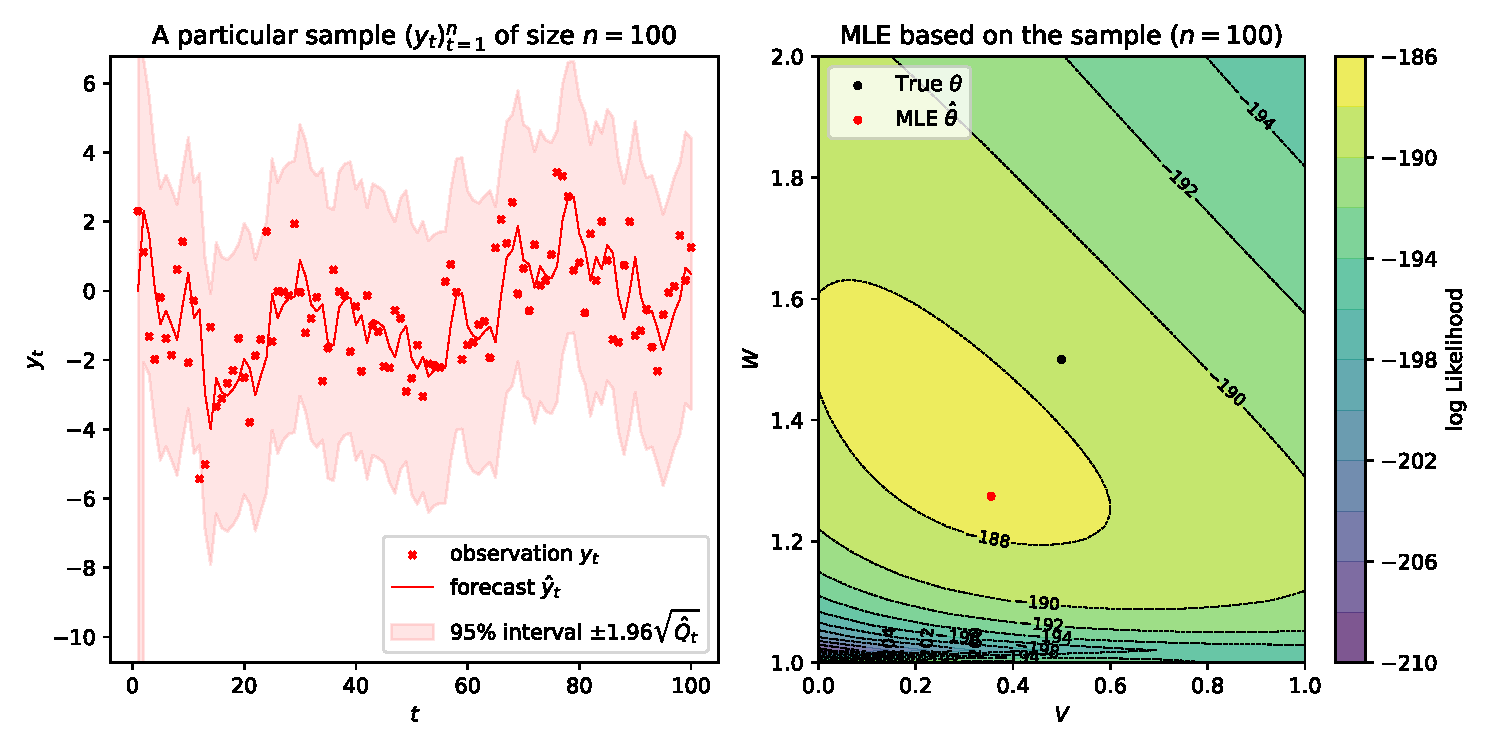
\includegraphics[width=480pt]{figures/fig_local_level_model_100.pdf}
    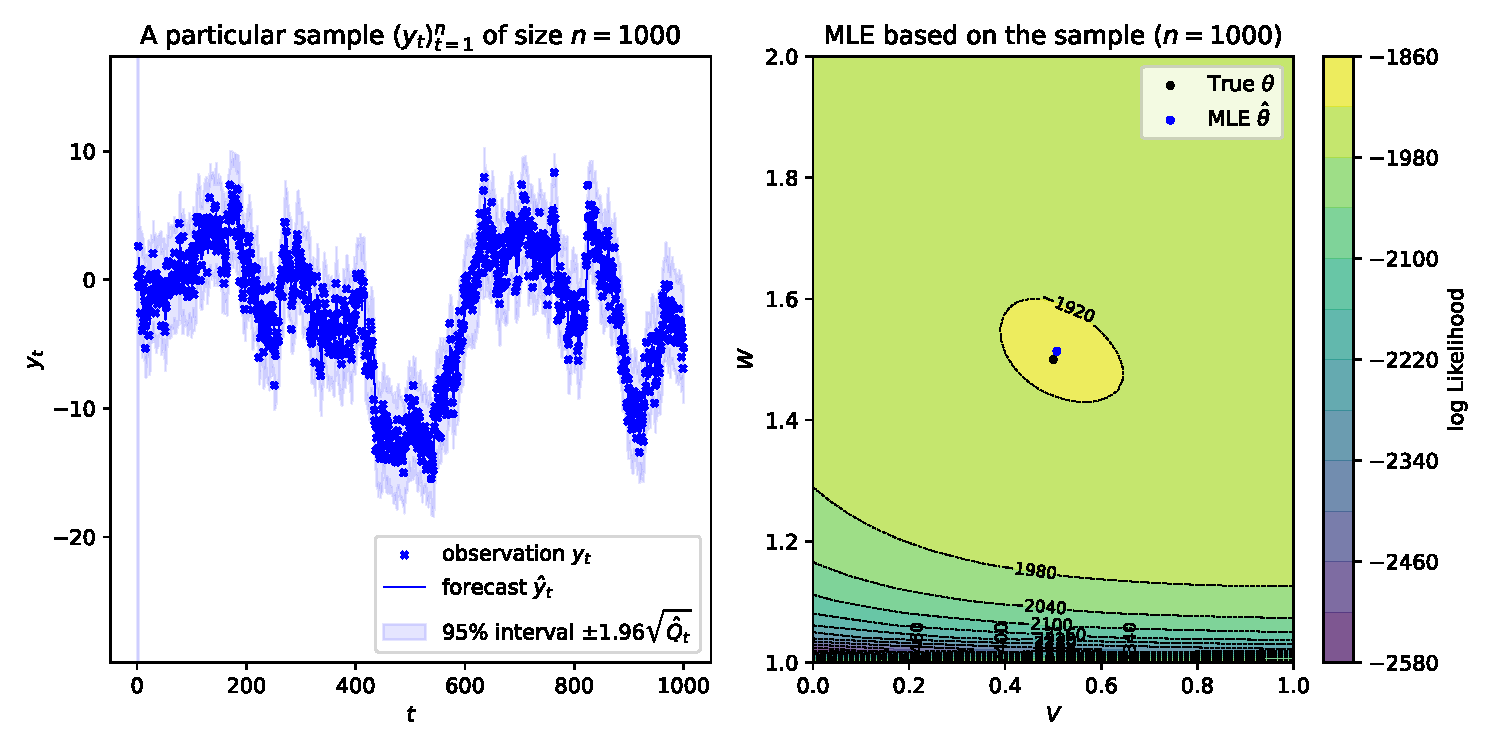
\includegraphics[width=480pt]{figures/fig_local_level_model_1000.pdf}
    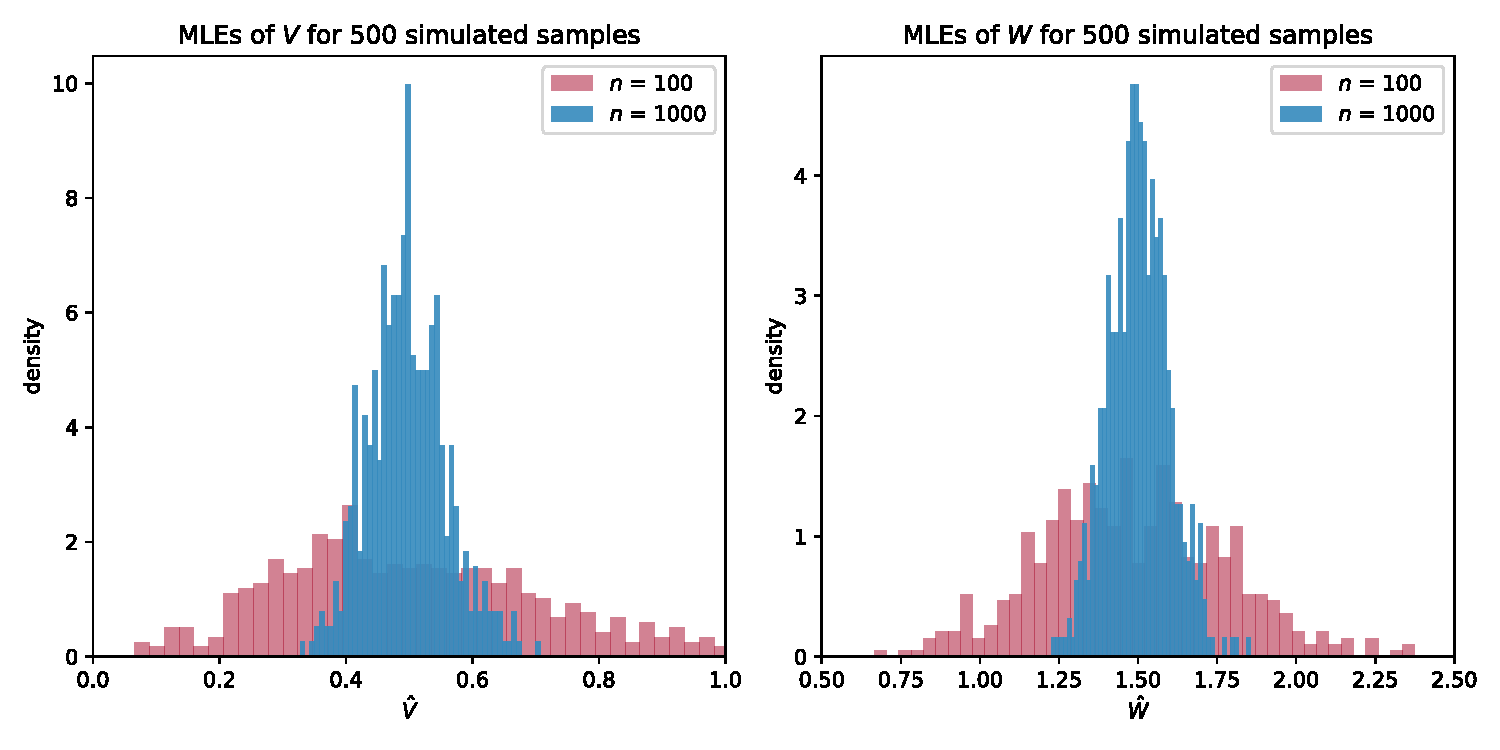
\includegraphics[width=465pt]{figures/fig_local_level_model_MLE_distribution.pdf}
    \caption{%
      Sample path $Y_{n}=(y_{1},\ldots, y_{n})$ generated from \eqref{eq:model_local} where $V=0.5, W=1.5$
      for different sample size, $n=100$ (top) or $n=1000$ (middle).
      The distribution of maximum likelihood estimator $\hat{V}, \hat{W}$ (bottom). 
    } 
    \label{fig:local_level}
  \end{figure} 

\end{itemize}

\clearpage

\section{General linear state-space model}

\subsection{Model}

\begin{itemize}

\item \textbf{Linear Gaussian state space model}
  \begin{itemize}
  \item Consider a time series $(\bm{y}_{t})_{t=1}^{n}$ from the following
    data generating process:
    \begin{equation}\label{eq:model_linear}%
      \begin{aligned}
        \bm{x}_{t} & = \bm{A}_{t}\bm{x}_{t-1} + \bm{v}_{t} + \bm{\nu}_{t}, \quad \bm{\nu}_{t}=\bm{V}_{t}^{\frac{1}{2}}\bm{z}_{\nu,t} \sim \mathcal{N}(\bm{0},\bm{V}_{t}) \\
        \bm{y}_{t} & =  \bm{C}_{t}\bm{x}_{t} + \bm{w}_{t} + \bm{\omega}_{t}, \quad \bm{\omega}_{t}=\bm{W}_{t}^{\frac{1}{2}}\bm{z}_{\omega,t} \sim \mathcal{N}(\bm{0},\bm{W}_{t}) \\
      \end{aligned}
      \qquad \forall t = 1, 2, \ldots, n,
    \end{equation}
    where $\bm{A}_{t}\in\R^{m\times m}$,
    $\bm{C}_{t}\in \R^{p\times m}$,
    $\bm{v}_{t}\in \R^{m}$, $\bm{w}_{t}\in\R^{p}$,
    $\bm{V}_{t}\in \R^{m\times m}$, $\bm{W}_{t}\in\R^{p\times p}$,
    and
    \begin{itemize}
    \item $\bm{x}_{t}\in\R^{m}$: potentially unobservable (latent)
      state vector at time~$t$
    \item $\bm{y}_{t}\in\R^{p}$: observed vector at time~$t$
    \item $\bm{\nu}_{t}\in\R^{m}$: state disturbance at time~$t$ (white
      noise)
    \item $\bm{\omega}_{t}\in\R^{p}$: observation disturbance at time~$t$
      (white noise)
    \end{itemize}

  \end{itemize}

\end{itemize}

\subsection{Kalman filter}

\begin{itemize}

\item \textbf{Filtering process}

  \begin{itemize}

  \item STEP~0: Initial state distribution
    \begin{itemize}
    \item Assume there exists a standard (multivariate) Gaussian
      $\bm{z}_{0}\sim \mathcal{N}(0,\bm{I})$ and
      \begin{equation}\label{eq:alpha0_linear}%
        \bm{x}_{0} = \bm{x}_{0|0} + \bm{P}_{0|0}^{\frac{1}{2}}\bm{z}_{0} \sim \mathcal{N} (\bm{x}_{0|0},\bm{P}_{0|0})
      \end{equation}
      for some known vector $\bm{x}_{0|0}\in \R^{m}$ and positive definite matrix $\bm{P}_{0|0}\in \R^{m\times m}$
    \end{itemize}

  \item STEP~1:
    Prior $\bm{x}_{1}|Y_{0}$,
    forecast $\bm{x}_{1}|Y_{0}$,
    and posterior $\bm{x}_{1}|Y_{1}$

    \begin{itemize}

    \item Given \eqref{eq:model_linear} and \eqref{eq:alpha0_linear},
      the joint distribution is
      \begin{align}
        \begin{bmatrix}
          \bm{x}_{1}|Y_{0}\\
          \bm{y}_{1}|Y_{0}\\
        \end{bmatrix}
        & =
          \begin{bmatrix}
            \bm{A}_{1}\bm{x}_{0}|Y_{0} + \bm{v}_{1} + \bm{\nu}_{1}\\
            \bm{C}_{1}\bm{x}_{1}|Y_{0} + \bm{w}_{1} + \bm{\omega}_{1}\\
          \end{bmatrix}
          \nonumber \\
        & =
          \begin{bmatrix}
            \bm{A}_{1}\bm{x}_{0|0} + \bm{v}_{1}\\
            \bm{C}_{1}\bm{A}_{1}\bm{x}_{0|0} + \bm{C}_{1}\bm{v}_{1} + \bm{w}_{1}
          \end{bmatrix}
          +
          \begin{bmatrix}
            \bm{A}_{1}\bm{P}_{0|0}^{\frac{1}{2}} & \bm{V}_{1}^{\frac{1}{2}} & \bm{O} \\
            \bm{C}_{1}\bm{A}_{1}\bm{P}_{0|0}^{\frac{1}{2}} & \bm{C}_{1}\bm{V}_{1}^{\frac{1}{2}} & \bm{W}_{1}^{\frac{1}{2}}\\
          \end{bmatrix}
          \begin{bmatrix}
            \bm{z}_{0}\\
            \bm{z}_{\nu,1}\\
            \bm{z}_{\omega,1}
          \end{bmatrix}
          \nonumber \\
          & ~ \sim
          \mathcal{N} \left(
          \begin{bmatrix}
            \bm{A}_{1}\bm{x}_{0|0} + \bm{v}_{1}\\
            \bm{C}_{1}\bm{A}_{1}\bm{x}_{0|0} + \bm{C}_{1}\bm{v}_{1} + \bm{w}_{1}
          \end{bmatrix},
          \bm{\Sigma}
          \right),
          \label{eq:alpha1y1Y0_linear}% 
      \end{align}
      where
      \begin{align}\nonumber%\label{eq:}%
        \bm{\Sigma}
        & =
          \begin{bmatrix}
            \bm{A}_{1}\bm{P}_{0|0}^{\frac{1}{2}} & \bm{V}_{1}^{\frac{1}{2}} & \bm{O}\\
            \bm{C}_{1}\bm{A}_{1}\bm{P}_{0|0}^{\frac{1}{2}} & \bm{C}_{1}\bm{V}_{1}^{\frac{1}{2}} & \bm{W}_{1}^{\frac{1}{2}}\\
          \end{bmatrix}
          \begin{bmatrix}
            (\bm{A}_{1}\bm{P}_{0|0}^{\frac{1}{2}})^{\top} & (\bm{C}_{1}\bm{A}_{1}\bm{P}_{0|0}^{\frac{1}{2}})^{\top}\\
            (\bm{V}_{1}^{\frac{1}{2}})^{\top} & (\bm{C}_{1}\bm{V}_{1}^{\frac{1}{2}})^{\top} \\
            \bm{O} & (\bm{W}_{1}^{\frac{1}{2}})^{\top} \\
          \end{bmatrix}
          \nonumber \\
        & = 
          \begin{bmatrix}
            \bm{A}_{1}\bm{P}_{0|0}\bm{A}_{1}^{\top} + \bm{V}_{1} & (\bm{A}_{1}\bm{P}_{0|0}\bm{A}_{1}^{\top} + \bm{V}_{1})\bm{C}_{1}^{\top}\\
            \bm{C}_{1}(\bm{A}_{1}\bm{P}_{0|0}\bm{A}_{1}^{\top} + \bm{V}_{1})^{\top} & \bm{C}_{1}(\bm{A}_{1}\bm{P}_{0|0}\bm{A}_{1}^{\top} + \bm{V}_{1})\bm{C}_{1}^{\top} + \bm{W}_{1}\\
          \end{bmatrix}
      \end{align}

    \item The prior on $\bm{x}_{1}$ and the forecast on $\bm{y}_{1}$ are therefore
      \begin{equation}\label{eq:alpha1Y0_linear}%
        \bm{x}_{1}|Y_{0}
        \sim \mathcal{N} \bigg(
        \underbrace{\bm{A}_{1}\bm{x}_{0|0} + \bm{v}_{1}}_{=:\hat{\bm{x}}_{1}},
        \underbrace{\bm{A}_{1}\bm{P}_{0|0}\bm{A}_{1}^{\top} + \bm{V}_{1}}_{=:\hat{\bm{P}}_{1}}
        \bigg),
        \quad
        \bm{y}_{1}|Y_{0}
        \sim \mathcal{N} \bigg(
        \underbrace{\bm{C}_{1}\hat{\bm{x}}_{1} + \bm{w}_{1}}_{=:\hat{\bm{y}}_{1}},
        \underbrace{\bm{C}_{1}\hat{\bm{P}}_{1}\bm{C}_{1}^{\top}+\bm{W}_{1}}_{=:\hat{\bm{Q}}_{1}}
        \bigg)
      \end{equation}

    \item Once $\bm{y}_{1}$ is observed, it follows from \eqref{eq:alpha1y1Y0_linear}
      that the posterior $\bm{x}_{1}|Y_{1}$ is\footnote{Here, just to make the expression easier to read,
        we introduce `division` of matrices as
        $\frac{X_{1}}{X_{2}} :=X_{1}X_{2}^{-1}$.}
      \begin{align}
        \bm{x}_{1}|Y_{1}
        & \sim
          \mathcal{N} \bigg(
          \bm{A}_{1}\bm{x}_{0|0} + \bm{v}_{1} + \frac{(\bm{A}_{1}\bm{P}_{0|0}\bm{A}_{1}^{\top} + \bm{V}_{1})\bm{C}_{1}^{\top}}{\bm{C}_{1}(\bm{A}_{1}\bm{P}_{0|0}\bm{A}_{1}^{\top} + \bm{V}_{1})\bm{C}_{1}^{\top} + \bm{W}_{1}}(\bm{y}_{1}-\bm{C}_{1}\bm{A}_{1}\bm{x}_{0|0} - \bm{C}_{1}\bm{v}_{1} - \bm{w}_{1}), \nonumber \\
        & \qquad\quad
          (\bm{A}_{1}\bm{P}_{0|0}\bm{A}_{1}^{\top} + \bm{V}_{1}) -\frac{(\bm{A}_{1}\bm{P}_{0|0}\bm{A}_{1}^{\top} + \bm{V}_{1})\bm{C}_{1}^{\top}}{\bm{C}_{1}(\bm{A}_{1}\bm{P}_{0|0}\bm{A}_{1}^{\top} + \bm{V}_{1})\bm{C}_{1}^{\top} + \bm{W}_{1}}\bm{C}_{1}(\bm{A}_{1}\bm{P}_{0|0}\bm{A}_{1}^{\top} + \bm{V}_{1})
          \bigg)
          \nonumber \\
        & =
          \mathcal{N} \bigg(
          \underbrace{\hat{\bm{x}}_{1} + \frac{\hat{\bm{P}}_{1}\bm{C}_{1}^{\top}}{\hat{\bm{Q}}_{1}}(\bm{y}_{1}-\hat{\bm{y}}_{1})}_{=:\bm{x}_{1|1}},
          \underbrace{\hat{\bm{P}}_{1} - \frac{\hat{\bm{P}}_{1}\bm{C}_{1}^{\top}}{\hat{\bm{Q}}_{1}}\hat{\bm{Q}}_{1}\left(\frac{\hat{\bm{P}}_{1}\bm{C}_{1}^{\top}}{\hat{\bm{Q}}_{1}}\right)^{\top}}_{=:\bm{P}_{1|1}}
          \bigg)
          \label{eq:alpha1Y1_linear}%
      \end{align}

    \item Note \eqref{eq:alpha1Y1_linear} may be written as
      \begin{equation}\label{eq:alpha1Y1z_linear}%
        \bm{x}_{1}|Y_{1} = \bm{x}_{1|1} + \bm{P}_{1|1}^{\frac{1}{2}}\bm{z}_{1},
      \end{equation}
      where $\bm{z}_{1}\sim \mathcal{N}(\bm{0},\bm{I})$ is independent of
      $(\bm{\nu}_{2},\bm{\omega}_{2})$ because it comes from
      $(\bm{z}_{0},\bm{\nu}_{1},\bm{\omega}_{1})$

    \end{itemize}

  \item STEP~2:
    Prior $\bm{x}_{2}|Y_{1}$,
    forecast $\bm{x}_{2}|Y_{1}$,
    and posterior $\bm{x}_{2}|Y_{2}$

    \begin{itemize}

    \item
      Using $\bm{x}_{1}|Y_{1}$ defined as \eqref{eq:alpha1Y1z_linear} and the model \eqref{eq:model_linear},
      we have
      \begin{align}
        \begin{bmatrix}
          \bm{x}_{2}|Y_{1}\\
          \bm{y}_{2}|Y_{1}\\
        \end{bmatrix}
        & =
          \begin{bmatrix}
            \bm{A}_{2}\bm{x}_{1}|Y_{1} + \bm{v}_{2} + \bm{\nu}_{2}\\
            \bm{C}_{2}\bm{x}_{2}|Y_{1} + \bm{w}_{2} + \bm{\omega}_{2}\\
          \end{bmatrix}
          \nonumber \\
        & =
          \begin{bmatrix}
            \bm{A}_{2}\bm{x}_{1|1} + \bm{v}_{2}\\
            \bm{C}_{2}\bm{A}_{2}\bm{x}_{1|1} + \bm{C}_{2}\bm{v}_{2} + \bm{w}_{2}
          \end{bmatrix}
          +
          \begin{bmatrix}
            \bm{A}_{2}\bm{P}_{1|1}^{\frac{1}{2}} & \bm{V}_{2}^{\frac{1}{2}} & \bm{O} \\
            \bm{C}_{2}\bm{A}_{2}\bm{P}_{1|1}^{\frac{1}{2}} & \bm{C}_{2}\bm{V}_{2}^{\frac{1}{2}} & \bm{W}_{2}^{\frac{1}{2}}\\
          \end{bmatrix}
          \begin{bmatrix}
            \bm{z}_{1}\\
            \bm{z}_{\nu,2}\\
            \bm{z}_{\omega,2}
          \end{bmatrix}
          \nonumber \\
          & ~ \sim
          \mathcal{N} \left(
          \begin{bmatrix}
            \bm{A}_{2}\bm{x}_{1|1} + \bm{v}_{2}\\
            \bm{C}_{2}\bm{A}_{2}\bm{x}_{1|1} + \bm{C}_{2}\bm{v}_{2} + \bm{w}_{2}
          \end{bmatrix},
          \bm{\Sigma}
          \right),
          \label{eq:alpha2y2Y1_linear}%
      \end{align}
      where
      \begin{equation}\nonumber%\label{eq:}%
        \bm{\Sigma}
        =
        \begin{bmatrix}
          \bm{A}_{2}\bm{P}_{1|1}\bm{A}_{2}^{\top} + \bm{V}_{2} & (\bm{A}_{2}\bm{P}_{1|1}\bm{A}_{2}^{\top} + \bm{V}_{2})\bm{C}_{2}^{\top}\\
          \bm{C}_{2}(\bm{A}_{2}\bm{P}_{1|1}\bm{A}_{2}^{\top} + \bm{V}_{2})^{\top} & \bm{C}_{2}(\bm{A}_{2}\bm{P}_{1|1}\bm{A}_{2}^{\top} + \bm{V}_{2})\bm{C}_{2}^{\top} + \bm{W}_{2}\\
        \end{bmatrix},
        \nonumber%\label{eq:}%
      \end{equation}
      from which we can compute the marginal distributions as
      \begin{equation}\nonumber%\label{eq:a2P2_linear}%
        \bm{x}_{2}|Y_{1}
        \sim \mathcal{N} \bigg(
        \underbrace{\bm{A}_{2}\bm{x}_{1|1} + \bm{v}_{2}}_{=:\hat{\bm{x}}_{2}},
        \underbrace{\bm{A}_{2}\bm{P}_{1|1}\bm{A}_{2}^{\top} + \bm{V}_{2}}_{=:\hat{\bm{P}}_{2}}
        \bigg),
        \quad
        \bm{y}_{2}|Y_{1}
        \sim \mathcal{N} \bigg(
        \underbrace{\bm{C}_{2}\hat{\bm{x}}_{2} + \bm{w}_{2}}_{=:\hat{\bm{y}}_{2}},
        \underbrace{\bm{C}_{2}\hat{\bm{P}}_{2}\bm{C}_{2}^{\top}+\bm{W}_{2}}_{=:\hat{\bm{Q}}_{2}}
        \bigg)
      \end{equation}

    \item Once $\bm{y}_{2}$ is observed, it follows from \eqref{eq:alpha2y2Y1_linear}
      that the posterior $\bm{x}_{2}|Y_{2}$ is
      \begin{align}
        \bm{x}_{2}|Y_{2}
        & \sim
          \mathcal{N} \bigg(
          \underbrace{\hat{\bm{x}}_{2} + \frac{\hat{\bm{P}}_{2}\bm{C}_{2}^{\top}}{\hat{\bm{Q}}_{2}}(\bm{y}_{2}-\hat{\bm{y}}_{2})}_{=:\bm{x}_{2|2}},
          \underbrace{\hat{\bm{P}}_{2} - \frac{\hat{\bm{P}}_{2}\bm{C}_{2}^{\top}}{\hat{\bm{Q}}_{2}}\hat{\bm{Q}}_{2}\left(\frac{\hat{\bm{P}}_{2}\bm{C}_{2}^{\top}}{\hat{\bm{Q}}_{2}}\right)^{\top}}_{=:\bm{P}_{2|2}}
          \bigg)
          \label{eq:alpha2Y2_linear}%
      \end{align}

    \item Note \eqref{eq:alpha2Y2_linear} may be written as
      \begin{equation}\label{eq:alpha2Y2z_linear}%
        \bm{x}_{2}|Y_{2} = \bm{x}_{2|2} + \bm{P}_{2|2}^{\frac{1}{2}}\bm{z}_{2},
      \end{equation}
      where $\bm{z}_{2}\sim \mathcal{N}(\bm{0},\bm{I})$ is independent of
      $(\bm{\nu}_{3},\bm{\omega}_{3})$

    \end{itemize}

  \item STEP~$t$:
    Prior $\bm{x}_{t}|Y_{t-1}$,
    forecast $\bm{x}_{t}|Y_{t-1}$,
    and posterior $\bm{x}_{t}|Y_{t}$

    \begin{itemize}

    \item Using $\bm{x}_{t-1}|Y_{t-1}$ (from the preceding step)
      and the model \eqref{eq:model_linear},
      we have
      \begin{align}
        \begin{bmatrix}
          \bm{x}_{t}|Y_{t-1}\\
          \bm{y}_{t}|Y_{t-1}\\
        \end{bmatrix}
        & =
          \begin{bmatrix}
            \bm{A}_{t}\bm{x}_{t-1}|Y_{t-1} + \bm{v}_{t} + \bm{\nu}_{t}\\
            \bm{C}_{t}\bm{x}_{t}|Y_{t-1} + \bm{w}_{t} + \bm{\omega}_{t}\\
          \end{bmatrix}
          \nonumber \\
        & =
          \begin{bmatrix}
            \bm{A}_{t}\bm{x}_{t-1|t-1} + \bm{v}_{t}\\
            \bm{C}_{t}\bm{A}_{t}\bm{x}_{t-1|t-1} + \bm{C}_{t}\bm{v}_{t} + \bm{w}_{t}
          \end{bmatrix}
          +
          \begin{bmatrix}
            \bm{A}_{t}\bm{P}_{t-1|t-1}^{\frac{1}{2}} & \bm{V}_{t}^{\frac{1}{2}} & \bm{O} \\
            \bm{C}_{t}\bm{A}_{t}\bm{P}_{t-1|t-1}^{\frac{1}{2}} & \bm{C}_{t}\bm{V}_{t}^{\frac{1}{2}} & \bm{W}_{t}^{\frac{1}{2}}\\
          \end{bmatrix}
          \begin{bmatrix}
            \bm{z}_{t-1}\\
            \bm{z}_{\nu,t}\\
            \bm{z}_{\omega,t}
          \end{bmatrix}
          \nonumber \\
          & ~ \sim
          \mathcal{N} \left(
          \begin{bmatrix}
            \bm{A}_{t}\bm{x}_{t-1|t-1} + \bm{v}_{t}\\
            \bm{C}_{t}\bm{A}_{t}\bm{x}_{t-1|t-1} + \bm{C}_{t}\bm{v}_{t} + \bm{w}_{t}
          \end{bmatrix},
          \bm{\Sigma}
          \right),
          \label{eq:alphatytYtm1_linear}%
      \end{align}
      where
      \begin{equation}\nonumber%\label{eq:}%
        \bm{\Sigma}
        =
        \begin{bmatrix}
          \bm{A}_{t}\bm{P}_{t-1|t-1}\bm{A}_{t}^{\top} + \bm{V}_{t} & (\bm{A}_{t}\bm{P}_{t-1|t-1}\bm{A}_{t}^{\top} + \bm{V}_{t})\bm{C}_{t}^{\top}\\
          \bm{C}_{t}(\bm{A}_{t}\bm{P}_{t-1|t-1}\bm{A}_{t}^{\top} + \bm{V}_{t})^{\top} & \bm{C}_{t}(\bm{A}_{t}\bm{P}_{t-1|t-1}\bm{A}_{t}^{\top} + \bm{V}_{t})\bm{C}_{t}^{\top} + \bm{W}_{t}\\
        \end{bmatrix},
        \nonumber%\label{eq:}%
      \end{equation}
      from which we can compute the marginal distributions as
      \begin{equation}\nonumber%\label{eq:a2P2_linear}%
        \bm{x}_{t}|Y_{t-1}
        \sim \mathcal{N} \bigg(
        \underbrace{\bm{A}_{t}\bm{x}_{t-1|t-1} + \bm{v}_{t}}_{=:\hat{\bm{x}}_{t}},
        \underbrace{\bm{A}_{t}\bm{P}_{t-1|t-1}\bm{A}_{t}^{\top} + \bm{V}_{t}}_{=:\hat{\bm{P}}_{t}}
        \bigg),
        \quad
        \bm{y}_{t}|Y_{t-1}
        \sim \mathcal{N} \bigg(
        \underbrace{\bm{C}_{t}\hat{\bm{x}}_{t} + \bm{w}_{t}}_{=:\hat{\bm{y}}_{t}},
        \underbrace{\bm{C}_{t}\hat{\bm{P}}_{t}\bm{C}_{t}^{\top}+\bm{W}_{t}}_{=:\hat{\bm{Q}}_{t}}
        \bigg)
      \end{equation}

    \item Once $\bm{y}_{t}$ is observed, it follows from \eqref{eq:alphatytYtm1_linear}
      that the posterior $\bm{x}_{t}|Y_{t}$ is
      \begin{align}
        \bm{x}_{t}|Y_{t}
        & \sim
          \mathcal{N} \bigg(
          \underbrace{\hat{\bm{x}}_{t} + \frac{\hat{\bm{P}}_{t}\bm{C}_{t}^{\top}}{\hat{\bm{Q}}_{t}}(\bm{y}_{t}-\hat{\bm{y}}_{t})}_{=:\bm{x}_{t|t}},
          \underbrace{\hat{\bm{P}}_{t} - \frac{\hat{\bm{P}}_{t}\bm{C}_{t}^{\top}}{\hat{\bm{Q}}_{t}}\hat{\bm{Q}}_{t}\left(\frac{\hat{\bm{P}}_{t}\bm{C}_{t}^{\top}}{\hat{\bm{Q}}_{t}}\right)^{\top}}_{=:\bm{P}_{t|t}}
          \bigg)
          \label{eq:alphatYt_linear}%
      \end{align}

    \end{itemize}

  \end{itemize}

\item \textbf{Kalman filter equations}

  \begin{itemize}

  \item Priors and posteriors can be incrementally computed in the
    following sequential manner:
    \begin{itemize}

    \item[1.] Given the posterior $\bm{x}_{t-1}|Y_{t-1}\sim \mathcal{N}(\bm{x}_{t-1|t-1},\bm{P}_{t-1|t-1})$ from the previous period,
      compute the prior:
      \begin{equation}\label{eq:KFE_atAt_linear}%
        \bm{x}_{t}|Y_{t-1}\sim \mathcal{N}(\hat{\bm{x}}_{t},\hat{\bm{P}}_{t})
        \quad\text{where}\quad
        \begin{aligned}
          \hat{\bm{x}}_{t} & = \bm{A}_{t}\bm{x}_{t-1|t-1} + \bm{v}_{t} \\
          \hat{\bm{P}}_{t} & = \bm{A}_{t}\bm{P}_{t-1|t-1}\bm{A}_{t}^{\top} + \bm{V}_{t} \\
        \end{aligned}
      \end{equation}

    \item[2.] Given the prior
      $\bm{x}_{t}|Y_{t-1}\sim \mathcal{N}(\hat{\bm{x}}_{t},\hat{\bm{P}}_{t})$,
      compute the forecast:
      \begin{equation}\label{eq:KFE_ftFt_linear}%
        \bm{y}_{t}|Y_{t-1}\sim \mathcal{N}(\hat{\bm{y}}_{t},\hat{\bm{Q}}_{t})
        \quad\text{where}\quad
        \begin{aligned}
          \hat{\bm{y}}_{t} & = \bm{C}_{t}\hat{\bm{x}}_{t} + \bm{w}_{t} \\
          \hat{\bm{Q}}_{t} & = \bm{C}_{t}\hat{\bm{P}}_{t}\bm{C}_{t}^{\top} + \bm{W}_{t} \\
        \end{aligned} 
      \end{equation}
    \item[3.] 
      Compute the Kalman gain
      \begin{equation}\label{eq:KFE_Kt_linear}%
        \bm{K}_{t} = \hat{\bm{P}}_{t}\bm{C}_{t}^{\top}\hat{\bm{Q}}_{t}^{-1}
      \end{equation}

    \item[4.] Once $\bm{y}_{t}$ is observed,
      compute forecast error $\hat{\bm{q}}_{t}$ as
      \begin{equation}\label{eq:KFE_et_linear}%
        \hat{\bm{q}}_{t} = \bm{y}_{t} - \hat{\bm{y}}_{t}
      \end{equation}
      and derive the posterior distribution
      \begin{equation}\label{eq:KFE_attAtt_linear}%
        \bm{x}_{t}|Y_{t}\sim \mathcal{N}(\bm{x}_{t|t},\bm{P}_{t|t})
        \quad\text{where}\quad
        \begin{aligned}
          \bm{x}_{t|t} & = \hat{\bm{x}}_{t} + \bm{K}_{t}\hat{\bm{q}}_{t} \\
          \bm{P}_{t|t} & = \hat{\bm{P}}_{t} - \bm{K}_{t}\hat{\bm{Q}}_{t}\bm{K}_{t}^{\top} \\
        \end{aligned}
      \end{equation}

    \end{itemize}

  \item
    Equations~\eqref{eq:KFE_atAt_linear}--\eqref{eq:KFE_attAtt_linear}
    are called the Kalman filter equations

  \end{itemize}

  \clearpage
\item \textbf{Initialization for stationary state process}

  \begin{itemize}

  \item Consider the case where $\bm{v}_{t}=\bm{v}$, $\bm{A}_{t}=\bm{A}$, and $\rho(\bm{A})<1$, where
    we define
    \begin{equation}\nonumber%\label{eq:}%
      \rho(\bm{A}) := \max_{\lambda \in \sigma(\bm{A})}|\lambda|
      \quad\text{where $\sigma(\bm{A})$ is the set of all eigenvalues of $\bm{A}$},
    \end{equation}
    which makes sure that $\bm{A}\neq \bm{I}$ and
    $\lim_{\tau\to\infty}\bm{A}^{\tau} = \bm{O}$

  \item Model~\eqref{eq:model_linear} suggests that for any $t$ and
    $\tau\geq 1$, we may write
    \begin{equation}
      \bm{x}_{t}
      = \bm{A}\bm{x}_{t-1} + \bm{v} + \bm{\nu}_{t}
      = \bm{A}(\bm{A}\bm{x}_{t-2} + \bm{v} + \bm{\nu}_{t-1}) + \bm{v} +\bm{\nu}_{t}
      = \bm{A}^{\tau}\bm{x}_{t-\tau} + \sum_{s=0}^{\tau-1}\bm{A}^{s}(\bm{v}+\bm{\nu}_{t-s}),
      \nonumber%\label{eq:}%
    \end{equation}
    which, since $\rho(\bm{A})<1$, may even be written as
    \begin{equation}\label{eq:alphat_stationary_linear}%
      \bm{x}_{t} = \sum_{s=0}^{\infty}\bm{A}^{s}(\bm{v}+\bm{\nu}_{t-s}) \quad \forall t
    \end{equation}

  \item Expression~\eqref{eq:alphat_stationary_linear} implies that
    $\bm{x}_{t}$ is a stationary process in the sense that
    \begin{equation}\label{eq:stationary_alphat_linear}%
      \E[\bm{x}_{t}] = \E[\bm{x}_{t-k}]
      \quad\text{and}\quad
      \V[\bm{x}_{t}] = \V[\bm{x}_{t-k}] \quad \forall k
    \end{equation}

  \item It follows from \eqref{eq:stationary_alphat_linear} and
    \eqref{eq:model_linear} that the unconditional mean and variance
    must satisfy
    \begin{equation}\nonumber%\label{eq:}%
      \E[\bm{x}_{t}] = \bm{A}\E[\bm{x}_{t}] + \E[\bm{\nu}_{t}],
      \quad
      \V[\bm{x}_{t}] = \bm{A}\V[\bm{x}_{t}]\bm{A}^{\top} + \V[\bm{\nu}_{t}],
      \quad \forall t = 0, 1, 2, \ldots
    \end{equation}
    which can be solved for $\E[\bm{x}_{t}]$ and $\V[\bm{x}_{t}]$ as\footnote{ Note that
      one can directly take the expectation of
      \eqref{eq:alphat_stationary_linear} and obtain
      \begin{equation}\nonumber%\label{eq:}%
        \E[\bm{x}_{t}]
        = \E \left[ \sum_{s=0}^{\infty}\bm{A}^{s}(\bm{v}+\bm{\nu}_{t-s}) \right] 
        = \sum_{s=0}^{\infty}\bm{A}^{s}\E \left[ \bm{v}+\bm{\nu}_{t-s} \right] =(\bm{I}-\bm{A})^{-1}\bm{v}.
      \end{equation}
      Similarly, directly taking the variance of
      \eqref{eq:alphat_stationary_linear} yields
      \begin{equation}\nonumber%\label{eq:}%
        \V[\bm{x}_{t}]
        = \V \left[ \sum_{s=0}^{\infty}\bm{A}^{s}(\bm{v}+\bm{\nu}_{t-s}) \right] 
        = \sum_{s=0}^{\infty}\V\left[ \bm{A}^{s}\bm{\nu}_{t-s} \right] 
        = \sum_{s=0}^{\infty}\bm{A}^{s}\V\left[\bm{\nu}_{t-s} \right] (\bm{A}^{s})^{\top}
        = \sum_{s=0}^{\infty}\bm{A}^{s}\bm{V}(\bm{A}^{s})^{\top},
      \end{equation}
      which, since $\rho(\bm{A}\otimes \bm{A})<1$ because of $\rho(\bm{A})<1$,
      implies
      \begin{equation}\nonumber%\label{eq:}%
        \vect(\V[\bm{x}_{t}])
        = \sum_{s=0}^{\infty}\vect(\bm{A}^{s}\bm{V}(\bm{A}^{s})^{\top})
        = \sum_{s=0}^{\infty}(\bm{A}^{s}\otimes \bm{A}^{s})\vect(\bm{V})
        = \sum_{s=0}^{\infty}(\bm{A}\otimes \bm{A})^{s}\vect(\bm{V})
        = (\bm{I} - \bm{A}\otimes \bm{A})^{-1}\vect(\bm{V})
      \end{equation}
    }
    \begin{equation}\nonumber%\label{eq:}%
      \E[\bm{x}_{t}] = (\bm{I}-\bm{A})^{-1}\bm{v},
      \quad
      \vect(\V[\bm{x}_{t}]) = (\bm{I} - \bm{A}\otimes \bm{A})^{-1}\vect(\bm{V})
      \quad \forall t = 0, 1, 2, \ldots
    \end{equation}

  \item Therefore, if the state process is stationary, we can use the
    following initial distribution:
    \begin{equation}\label{eq:bmx0}%
      \bm{x}_{0}
      \sim
      \mathcal{N} \left(\E[\bm{x}_{0}], \V[\bm{x}_{0}]\right)
      =
      \mathcal{N} \left((\bm{I}-\bm{A})^{-1}\bm{v}, \vect_{m\times m}^{-1}((\bm{I} - \bm{A}\otimes \bm{A})^{-1}\vect(\bm{V}))\right)
    \end{equation}

  \end{itemize}

\item \textbf{Initialization for non-stationary state process}

  \begin{itemize}
  \item If the state process is non-stationary, then the strategy
    described above does not work, in which case we use the
    (approximate) uninformative prior

  \item To be more precise, we put $\bm{P}_{0|0}=\kappa \bm{I}$ and use a
    sufficiently large $\kappa\in \R$
  \end{itemize}

\end{itemize}

\clearpage
\subsection{Parameter estimation}

\begin{itemize}

\item \textbf{Maximum likelihood estimator}

  \begin{itemize}

  \item In case (some of) the model parameters
    $\bm{\theta}:=(\bm{A}_{t}, \bm{B}_{t}, \bm{C}_{t}, \bm{w}_{t}, \bm{V}_{t}, \bm{W}_{t})_{t\geq 1}$ are unknown, we
    estimate them as follows

  \item The joint distribution of $Y_{n}:=(\bm{y}_{1},\bm{y}_{2},\ldots, \bm{y}_{n})$
    is
    \begin{equation}\label{eq:PYt_linear}%
      p(Y_{n})
      = p(\bm{y}_{n}|Y_{n-1})p(Y_{n-1})
      = p(\bm{y}_{n}|Y_{n-1})p(\bm{y}_{n-1}|Y_{n-2})p(Y_{n-2})
      = \prod_{t=1}^{n}p(\bm{y}_{t}|Y_{t-1}),
    \end{equation}
    where \eqref{eq:KFE_ftFt_linear} implies
    \begin{align}\label{eq:pytYt1_linear}%
      p(\bm{y}_{t}|Y_{t-1})
      & = \frac{1}{(2\pi)^{\frac{p}{2}}|\hat{\bm{Q}}_{t}|^{\frac{1}{2}}}e^{- \frac{1}{2}(\bm{y}_{t}-\hat{\bm{y}}_{t})^{\top}\hat{\bm{Q}}_{t}^{-1}(\bm{y}_{t}-\hat{\bm{y}}_{t})}
    \end{align}

  \item MLE of $\bm{\theta}$ is the one that maximizes the log likelihood
    \begin{align}
      \ln L(\bm{\theta};Y_{n})
      & := \ln \left(p(Y_{n})\right)
        = \sum_{t=1}^{n}\ln \left(p(\bm{y}_{t}|Y_{t-1})\right) \nonumber \\
      & = \sum_{t=1}^{n}\left(- \frac{p}{2}\ln(2\pi) - \frac{1}{2}\ln(|\hat{\bm{Q}}_{t}|) - \frac{1}{2}(\bm{y}_{t}-\hat{\bm{y}}_{t})^{\top}\hat{\bm{Q}}_{t}^{-1}(\bm{y}_{t}-\hat{\bm{y}}_{t})\right) \nonumber \\
      & = - \frac{np}{2}\ln(2\pi) - \frac{1}{2}\sum_{t=1}^{n}\left(\ln(|\hat{\bm{Q}}_{t}|) +(\bm{y}_{t}-\hat{\bm{y}}_{t})^{\top}\hat{\bm{Q}}_{t}^{-1}(\bm{y}_{t}-\hat{\bm{y}}_{t})\right)
        \label{eq:logL_local_linear}%
    \end{align}
    
  \end{itemize}

\item \textbf{Example}

  \begin{itemize}
  \item Consider the case where
    the evolution of state vector, $\bm{x}_{t}=(x_{1,t},x_{2,t},x_{3,t})$,
    is governed by the following dynamical system:
    \begin{equation}\nonumber%\label{eq:}%
      \begin{bmatrix}
        x_{1,t} \\
        x_{2,t} \\
        x_{3,t} \\
      \end{bmatrix}
      =
      \begin{bmatrix}
        a_{11} & 0 & 0 \\
        a_{21} & a_{22} & a_{23} \\
        0 & a_{32} & a_{33} \\
      \end{bmatrix}
      \begin{bmatrix}
        x_{1,t-1} \\
        x_{2,t-1} \\
        x_{3,t-1} \\
      \end{bmatrix}
      +
      \begin{bmatrix}
        b \\
        0 \\
        0 \\
      \end{bmatrix}
      u_{t}
      + 
      \begin{bmatrix}
        \nu_{1,t} \\
        \nu_{2,t} \\
        \nu_{3,t} \\
      \end{bmatrix}
    \end{equation}
    where
    \begin{equation}\nonumber%\label{eq:}%
      \begin{bmatrix}
        \nu_{1,t} \\
        \nu_{2,t} \\
        \nu_{3,t} \\
      \end{bmatrix}
      \sim \mathcal{N}
      \left(
        \begin{bmatrix}
          0 \\
          0 \\
          0 \\
        \end{bmatrix},
        \begin{bmatrix}
          \sigma_{1}^{2} & 0 & 0 \\
          0 & \sigma_{2}^{2} & 0 \\
          0 & 0 & \sigma_{3}^{2} \\
        \end{bmatrix}
      \right)
    \end{equation}
  \item Suppose that we know that the unit step forcing is introduced after time $t=1$:
    \begin{equation}\nonumber%\label{eq:}%
      u_{t} =
      \begin{cases}
        1 & t \geq 1 \\
        0 & t \leq 0 \\
      \end{cases}
    \end{equation}
  \item Assume that:
    \begin{itemize}
    \item we can observe the value of $x_{2,t}$ for $t\geq 1$
    \item the values of $x_{1,t}$ and $x_{3,t}$
      are not directly observable, but we can observe the sum $\sum_{i=1}^{3}x_{i,t}$
    \item there is no measurement error
    \end{itemize}
  \item So the measurement vector $\bm{y}_{t}=(y_{1,t}, y_{2,t})$ is given by
    \begin{equation}\nonumber%\label{eq:}%
      \begin{bmatrix}
        y_{1,t} \\
        y_{2,t} \\
      \end{bmatrix}
      =
      \begin{bmatrix}
        0 & 1 & 0 \\
        1 & 1 & 1 \\
      \end{bmatrix}
      \begin{bmatrix}
        x_{1,t} \\
        x_{2,t} \\
        x_{3,t} \\
      \end{bmatrix}
      \quad \forall t = 1, 2, \ldots, n
    \end{equation}
  \item We want to estimate the value of $\bm{\theta}=(a_{11}, a_{21}, a_{22}, a_{23}, a_{32}, a_{33}, b, \sigma_{1}, \sigma_{2}, \sigma_{3})$
    based on the sample $Y_{n}=(\bm{y}_{1},\ldots, \bm{y}_{n})$ of size $n$

  \clearpage
  \begin{figure}[t]\centering%
    \includegraphics[width=475pt]%
    {figures/fig_linear_model.png}
    \caption{%
      Pairs plot of MLE $\hat{\bm{\theta}}$ (1000 simulated samples of size $n=250$).
    } 
    \label{fig:linear_model}
  \end{figure} 

\item \figurename~\ref{fig:linear_model} shows the estimated values of $\bm{\theta}$, where
  \begin{itemize}
  \item[1.] I first fix the true parameter values $\bm{\theta}$ as listed in the figure
    (the model is stationary because $\rho(\bm{A}) < 1$)
  \item[2.] Using this true $\bm{\theta}$, I generate a simulated sample $Y_{n}=(\bm{y}_{1},\ldots, \bm{y}_{n})$ of size $n$:
    \begin{itemize}
    \item randomly draw an initial state $\bm{x}_{0}$ based on \eqref{eq:bmx0} with $\bm{v}=\bm{0}$ (since $u_{t}=0$ for all $t\leq 0$)
    \item then randomly draw $\bm{\nu}_{1}$ and compute $\bm{x}_{1}$, which in turn determines $\bm{y}_{1}$
    \item then randomly draw $\bm{\nu}_{2}$ and compute $\bm{x}_{2}$, which in turn determines $\bm{y}_{2}$
    \item \ldots
    \end{itemize}
  \item[3.] For each $\tilde{\bm{\theta}}$, I combine the sample $Y_{n}$ and the Kalman filter equations~\eqref{eq:KFE_atAt_linear}--\eqref{eq:KFE_attAtt_linear}
    to compute its log likelihood $\ln(L(\tilde{\bm{\theta}};Y_{n}))$ based on \eqref{eq:logL_local_linear}
    and find the one that maximizes it:
    \begin{equation}\nonumber%\label{eq:}%
      \hat{\bm{\theta}} = \arg\max_{\tilde{\bm{\theta}}} \ln(L(\tilde{\bm{\theta}};Y_{n})) 
    \end{equation}
  \item[4.] I repeat Steps~2-3 for 1000 times to generate the simulated distribution of $\hat{\bm{\theta}}$
  \end{itemize}
    
  \end{itemize}

\end{itemize}

\end{document}
